\documentclass{article}
\usepackage{hyperref}
\usepackage{Style}

\nocite{*} % Comentar si quiero citar
%\addbibresource{bibliografia.bib} % Quitar el comentado si quiero usar bibliografia

\begin{document}

\begin{minipage}{2.5cm}
    \includegraphics[width=2cm]{imagen_puc.jpg}
\end{minipage}
\begin{minipage}{14cm}
    {\sc Pontificia Universidad Católica de Chile\\
    Facultad de Matemáticas\\
    Departamento de Matemática\\
    Profesor: Mauricio Bustamante -- Estudiante: Benjamín Mateluna}
\end{minipage}
\vspace{1ex}

{\centerline{\bf Topología Algebraica - MAT2850}
\centerline{\bf Apuntes}}
\centerline{\bf 05 de agosto de 2025}

\newpage
\tableofcontents

\newpage
\section*{Motivación}
\phantomsection
\addcontentsline{toc}{section}{Motivación}
\noindent Dados dos espacios topológicos $X$ e $Y$ ¿Cuando son homeomorfos?. Decimos que dos 
espacios son \textbf{homeomorfos} si existe $f:X\to Y$ continua, biyectiva y con inversa 
constinua. La topología algebraica ataca esta pregunta de la siguiente forma:
\begin{enumerate}
    \item Asigna a cada espacio topológico $X$ un objeto algebraico $G(X)$.
    \item Aigna a cada función continua $f:X\to Y$ un homomorfismo $G(f):G(X)\to G(Y)$ tal que
    \begin{enumerate}
        \item $G(f\circ g)=G(f)\circ G(g)$
        \item $G(id_{X})=id_{G(X)}$
    \end{enumerate}
\end{enumerate}
\noindent\textbf{Observación:} Ambas condiciones implican que si $f:X\to Y$ es homeomorfismo, 
entonces $G(f):G(X)\to G(Y)$ es isomorfismo. A veces los $G$ que se construyen satisfacen la 
propiedad extra que si $X$ se puede ''deformar continuamente'' en $Y$ entonces $G(X)\cong G(Y)$.

\vspace{2mm}
\noindent Decimos que $G$ es un \textbf{invariante homotópico}.

\noindent\textbf{Ejemplos:}
\begin{enumerate}
    \item Tenemos los espacios
    \begin{center} %Ilustraciones de la esfera y el toro
        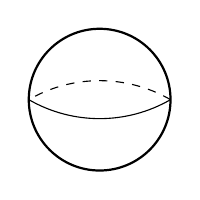
\begin{tikzpicture}[scale=0.9]
            \coordinate (A) at (0,0,0);
            \coordinate (B) at (-1,0,0);
            \coordinate (C) at (1,0,0);

            \filldraw[color=black, fill=white, thick] (A) circle (1);
            \draw (B) arc (240:300:2);
            \draw[dashed] (C) arc (60:120:2);
        \end{tikzpicture}
        %
        \hspace{2cm}
        %
        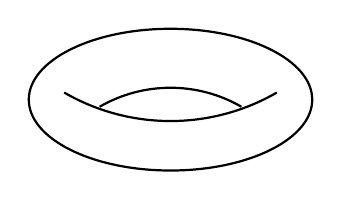
\begin{tikzpicture}[scale=0.9]
            \coordinate (A) at (0,0);
            \coordinate (B) at (-1.5,0.1);
            \coordinate (C) at (1,-0.1);

            \draw[thick] (A) ellipse (2cm and 1cm);
            \draw[thick] (B) arc (240:300:3);
            \draw[thick] (C) arc (60:120:2);
        \end{tikzpicture}
    \end{center}
    Mas adelante veremos que la homología le asigna a la esfera el grupo $\{e\}$ y al toro 
    $\Z^{2}$. En general, una superficie de genero $g$ tendrá el grupo $\Z^{2g}$.

    \item ¿Cuando $\R^{n}$ y $\R^{m}$ son homeomorfos? Si $n\neq$, el grupo de homología de 
    $\R^{n}$ será $\{e\}$ y por el contrario, para $\R^{m}$ va a ser $\Z$ y por lo tanto $R^{n}$ y
    $\R^{m}$ son homeomorfos si y solo si $n=m$.

    \item Un ejemplo particular, para el circulo se tiene que $\pi_{1}(\s^{1})=\Z$ pero 
    $\pi_{1}(\s^{2})=\{e\}$ y por lo tanto los espacios no son homeomorfos.
\end{enumerate}

\vspace{2mm}
\begin{dfn}
    Una \textbf{homotopía} entre dos funciones continuas $f,g:X\to Y$ es una función continua 
    $H:X\times[0,1]\to Y$ tal que $H(x,0)=f(x)$ y $H(x,1)=g(x)$ para todo $x\in X$.
\end{dfn}
\noindent\textbf{Notación:} La función $H_{t}:X\to Y$ esta dada por $H_{t}(x):=H(x,t)$. Una 
homotopía de $f$ a $g$ se denota por $f\sim g$.

\vspace{2mm}
\begin{prop}
    Ser homotópico es una relación de equivalencia en $\mathcal{C}(X,Y)$.
\end{prop}
\begin{proof}
    Debemos probar tres cosas
    \begin{enumerate}
        \item La relación es reflexiva. Sea $f:X\to Y$, consideramos la homotopía constante, esto
        es $H(x,t):=f(x)$ es continua ya que

        \centerline{
            \xymatrix{
                X\times[0,1] \ar[r]^-{\pi_{X}} \ar@/_0.8pc/[rr]_{H} & X \ar[r]^-{f} & Y
            }
        }
        \item Simetría. Supongamos que $f\sim g$, consideramos $H'(x,t)=H(x,1-t)$ y es continua
        por que
        
        \vspace{2mm}
        \centerline{
            \xymatrixcolsep{3pc}\xymatrix{
                X\times[0,1] \ar[r]^-{id\times(1-t)} \ar@/_1.1pc/[rr]_{H'} & X\times[0,1]
                \ar[r]^-{H} & Y
            }
        }
        \item Por último, la transitividad. Sean $f\sim g$ y $g\sim h$, Definimos 
        $H*G:X\times[0,1]\to Y$ dada por
        \begin{equation*}
            H*G(x,t):=\begin{cases}
                H(x,2t) &\quad\text{ si}\hspace{2mm}0\leq t\leq\frac{1}{2} \\
                G(x,2t-1) &\quad\text{ si}\hspace{2mm}\frac{1}{2}\leq t\leq1
            \end{cases}
        \end{equation*}
        que resulta continua por el lema del pegado.
    \end{enumerate}
\end{proof}

\newpage
\vspace{2mm}
\begin{dfn}
    Decimos que $f:X\to Y$ es una \textbf{equivalencia homotópica}, si existe $g:Y\to X$ tal que 
    $g\circ f\sim id_{X}$ y $f\circ g\sim id_{Y}$
\end{dfn}
\noindent En tal caso, $X$ e $Y$ se dicen homotópicamente equivalentes o que tienen el mismo tipo 
de homotopía y se denota por $X\sim Y$.

\vspace{2mm}
\noindent\textbf{Ejemplo:}
\begin{enumerate}
    \item Sea $f:X\to Y$ un homeomorfismo, en particular, tomando $g=f^{-1}$, se sigue que es 
    equivalencia homotópica.

    \item Se tiene que $\{0\}\sim\R^{n}$, consideremos la inclusión $i:\to\{0\}\to\R^{n}$, 
    afirmamos que es $i$ es equivalencia homotópica. En efecto, se verifica que $\pi:\R^{n}\to
    \{0\}$ es una inversa homotópica. Por un lado $\pi\circ i=id_{\{0\}}$ y por otro 
    $i\circ\pi=0$. Notamos que $H(x,t)=tx$ con $t\in[0,1]$ es una homotopía entre $0$ y 
    $id_{\R^{n}}$.

    \item Veamos que $\R^{n}\setminus\{0\}\sim\s^{n-1}$. Probaremos que la función 
    $i:\s^{n-1}\to\R^{n}\setminus\{0\}$ es equivalencia homotópica. En efecto,
    \begin{align*}
        \pi:\R^{n}\setminus\{0\} &\to \s^{n-1} \\
        x &\to \frac{x}{\abs{x}}
    \end{align*}
    es inversa homotópica. Es claro que $\pi\circ i=id_{s^{n-1}}$. Definimos
    \begin{equation*}
        H(x,t):=t\frac{x}{\abs{x}}+(1-t)x
    \end{equation*}
    Notamos que $H(x,0)=x$ y $H(x,1)=\frac{x}{\abs{x}}$, es decir, $H$ es una homotopia entre 
    $i\circ\pi$ e $id_{\R^{n}\setminus\{0\}}$. Además, se verifica que 
    $im(H)\subseteq\R^{n}\setminus\{0\}$.
\end{enumerate}

\newpage
\section{Homología}
\noindent Queremos asignarle a un espacio topológico $X$ arbitrario, grupos abelianos 
$H_{0}(X),H_{1}(X),\cdots$ tal que si $X\sim Y$, entonces $H_{i}(X)\cong H_{i}(Y)$ para todo $i$.
Ituitivamente, $H_{k}(X)$ estará generado por ciertos subespacios de $X$ de dimensión $k$.

\vspace{2mm}
\noindent Habrá una relación de equvalencia, $A,B\subseteq X$ de dimensión $k$ serán equivalentes
si hay un subespacio de $X$ de dimensión $k+1$ cuyo borde es $A\cup B$.

\vspace{2mm}
\noindent Hay que restringir la clase de espacios a una con nociones de dimensión, borde, etc. 
Estos serán los complejos simpliciales. Necesitamos, adicionalmente, un objeto algebraico que 
capture esas nociones, esto corresponde a los complejos de cadenas.

\subsection{Complejos de Cadenas}
\begin{dfn}
    Un \textbf{complejo de cadenas} es una sucesión de grupos abelianos y homomorfismos
    
    \vspace{2mm}
    \centerline{
        \xymatrix{
            \cdots \ar[r] & C_{3} \ar[r]^{\partial_{3}} & C_{2} \ar[r]^{\partial_{2}} & 
            C_{1} \ar[r]^{\partial_{1}} & C_{0} \ar[r] & 0
        }
    }
    \vspace{2mm}
    \noindent tal que $\partial_{i}\circ \partial_{i+1}=0$ para todo $i$. Se denota por 
    $(C_{\sbullet},\partial_{\sbullet})$.
\end{dfn}
\noindent\textbf{Observación:} Notemos que $\im{\partial_{i+1}}\subseteq\kr{\partial_{i}}
\subseteq C_{i}$. Dado que los grupos son abelianos, esta observación permite definir el siguiente 
objeto.

\vspace{2mm}
\begin{dfn}
    El \textbf{i-ésimo grupo de homología} de $(C_{\sbullet},\partial_{\sbullet})$ se define por
    \begin{equation*}
        H_{i}(C_{i}):=\frac{\kr{\partial_{i}}}{\im{\partial_{i+1}}}
    \end{equation*}
\end{dfn}

\vspace{2mm}
\noindent\textbf{Ejemplos:}
\begin{itemize}
    \item Si $A$ un grupo abeliano, entonces
    
    \vspace{2mm}
    \centerline{
        \xymatrix{
            \cdots \ar[r] & 0 \ar[r] & 0 \ar[r] & A \ar[r] & 0 \ar[r] & \cdots \ar[r] & 0
        }
    }
    \vspace{2mm}
    es un complejo de cadenas donde $C_{i}=A$. Entonces
    \begin{equation*}
        H_{j}(C_{\sbullet})=\begin{cases}
            0 & \quad\text{si }j\neq i \\
            A & \quad\text{si }j=i
        \end{cases}
    \end{equation*}

    \item Consideremos la cadena exacta
    
    \vspace{2mm}
    \centerline{
        \xymatrix{
            \cdots \ar[r] & 0 \ar[r] & \Z \ar[r]^{\cdot2} & \Z \ar[r]^{\pi} & \Z_{2} \ar[r] & 0
        }
    }
    \vspace{2mm}
    entonces $H_{j}(C_{\sbullet})=0$ para todo $i$.

    \item Veamos que
    
    \vspace{2mm}
    \centerline{
        \xymatrix{
            \cdots \ar[r] & \Z \ar[r]^{\cdot2} & \Z \ar[r]^{\cdot0} & \Z \ar[r] & 0
        }
    }
    \vspace{2mm}    
    es un complejo de cadenas. La homología asociadas son $H_{0}(C_{\sbullet})=\Z$, 
    $H_{1}(C_{\sbullet})=\Z_{2}$ y $H_{k}(C_{\sbullet})=0$.
\end{itemize}

\begin{dfn}
    Sean $(C_{\sbullet},\partial_{\sbullet})$ y $(D_{\sbullet},\partial_{\sbullet})$ dos complejos 
    de cadenas. Un \textbf{mapeo de cadenas} es una colección de homomorfismos 
    $f_{n}:C_{n}\to D_{n}$ tal que $\partial_{n}f_{n}=f_{n-1}\partial_{n}$ para todo $n$, es 
    decir, el siguiente diagrama conmuta

    \vspace{2mm}
    \centerline{
        \xymatrix{
            C_{n} \ar[r]^{\partial_{n}} \ar[d]^{f_{n}} & C_{n-1} \ar[d]^{f_{n-1}} \\
            D_{n} \ar[r]^{\partial_{n}} & D_{n-1}
        }
    }
    \noindent y se denota por $f_{\sbullet}:C_{\sbullet}\to D_{\sbullet}$.
\end{dfn}

\vspace{2mm}
\begin{lema}
    Si $f_{\sbullet}:C_{\sbullet}\to D_{\sbullet}$ es un mapeo de cadenas, entonces la asignación 
    $f_{*}:H_{n}(C_{\sbullet})\to H_{n}(D_{\sbullet})$ dada por
    \begin{equation*}
        f_{*}([x])=[f_{n}(x)]
    \end{equation*}
    esta bien definida y es un homomorfismo de grupos.
\end{lema}
\begin{proof}
    Sea $x\in ker\partial_{n}$ entonces $\partial_{n}f_{n}(x)=f_{n-1}\partial_{n}(x)
    =f_{n-1}(0)=0$. Así, $f_{n}(x)\in\kr{\partial_{n}}$ y por tanto la expresión tiene sentido. Si
    $[x]=[y]$ entonces $x-y=\partial_{n}(z)$ para $z\in C_{n+1}$, se sigue que 
    $f_{n}(x)-f_{n}(y)=f_{n}\partial_{n+1}(z)=\partial_{n+1}f_{n+1}(z)$. Concluimos que 
    $[f_{n}(x)]=[f_{n}(y)]$.
\end{proof}

\noindent\textbf{Ejemplo:}
Consideremos la siguiente situación

\vspace{2mm}
\centerline{
    \xymatrix{
        \cdots \ar[r] & 0 \ar[r]^{0} \ar[d] & \Z \ar[r]^{3} \ar[d]^{id} & 
        \Z \ar[r]^{0} \ar[d]^{\pi} & \Z \ar[r] \ar[d]^{id} & 0 
        & C_{\sbullet} \ar[d]^{f_{\sbullet}} \\
        \cdots \ar[r] & 0 \ar[r]^{0} & \Z \ar[r]^{3} & \Z_{3} \ar[r]^{0} & \Z \ar[r] & 0 
        & D_{\sbullet}
    }
}
\vspace{2mm}
\noindent Entonces $f_{*}:H_{2}(C_{\sbullet})=0\to H_{2}(D_{\sbullet})=\Z$ es el morfismo trivial. 
Mientras que $\pi_{*}:H_{1}(C_{\sbullet})=\Z_{3}\to H_{1}(D_{\sbullet})=\Z_{3}$ es la identidad.

\vspace{2mm}
\noindent\textbf{Observación:} Sea $g_{\sbullet}:D_{\sbullet}\to G_{\sbullet}$ un mapeo de 
cadenas, entonces $(g\circ f)_{\sbullet}:C_{\sbullet}\to G_{\sbullet}$ es un mapeo de cadenas y el 
siguiente diagrama conmuta

\vspace{2mm}
\centerline{
    \xymatrix{
        H_{n}(C_{\sbullet}) \ar[rr]^{(g\circ f)_{*}} \ar[rd]^{f_{*}} & 
        & H_{n}(G_{\sbullet}) \\
        & H_{n}(D_{\sbullet}) \ar[ru]^{g_{*}}
    }
}
\vspace{2mm}
\noindent Notemos que $\partial_{n}g_{n} f_{n}=g_{n-1}\partial_{n}f_{n}=g_{n-1}f_{n-1}
\partial_{n}$. Por otro lado, tenemos que $(g\circ f)_{*}([x])=[(g\circ f)(x)]=g_{*}([f(x)])=
(g_{*}\circ f_{*})([x])$, lo que prueba la afirmación.

\begin{dfn}
    Sean $i_{\sbullet}:A_{\sbullet}\to B_{\sbullet}$ y $j_{\sbullet}:B_{\sbullet}\to C_{\sbullet}$
    dos mapeos de cadenas. Decimos que forman una sucesión exacta corta si la secuencia

    \vspace{2mm}
    \centerline{
        \xymatrix{
            0 \ar[r] & A_{n} \ar[r]^{i_{n}} & B_{n} \ar[r]^{j_{n}} & C_{n} \ar[r] & 0
        }
    }
    \vspace{2mm}
    \noindent es exacta y corta de grupos abelianos libres para todo $n\in\N$. Lo denotamos como
    $0\to A_{\sbullet}\to B_{\sbullet}\to C_{\sbullet}\to0$.
\end{dfn}

\begin{teo}[Lema de la serpiente]
    Sea $0\to A_{\sbullet}\to B_{\sbullet}\to C_{\sbullet}\to0$ una secuencia de complejos de 
    cadenas, entonces existen morfismos
    \begin{equation*}
        \delta_{n}:H_{n}(C_{\sbullet})\to H_{n-1}(A_{\sbullet})
    \end{equation*}
    tal que
    
    \vspace{2mm}
    \centerline{
        \xymatrix{
            \ar[r]^-{\delta_{n+1}} & H_{n}(A_{\sbullet}) \ar[r]^{i_{*}} 
            & H_{n}(B_{\sbullet}) \ar[r]^{j_{*}} & H_{n}(C_{\sbullet}) 
            \ar `[dl] `[l] `[llld]_{\delta_{n}} `[d] [dll] \\
            & H_{n-1}(A_{\sbullet}) \ar[r]^{i_{*}} & H_{n-1}(B_{\sbullet}) \ar[r]^{j_{*}} 
            & H_{n-1}(C_{\sbullet}) \ar[r] & \cdots \\
            & \cdots \ar[r] & H_{0}(B_{\sbullet}) \ar[r] & H_{0}(C_{\sbullet}) \ar[r] & 0 
        }
    }
\end{teo}

\begin{proof}
    Vamos a hacer un cacería de diagramas (:D). Consideremos el diagrama

    \vspace{2mm}
    \centerline{
        \xymatrix{
            & \vdots \ar[d] & \vdots \ar[d] & \vdots \ar[d] & \\
            0 \ar[r] & A_{n+1} \ar[r]^{i} \ar[d]^{\partial} & B_{n+1} \ar[r]^{j} \ar[d]^{\partial} 
            & C_{n+1} \ar[r] \ar[d]^{\partial} & 0 \\
            0 \ar[r] & A_{n} \ar[r]^{i} \ar[d]^{\partial} & B_{n} \ar[r]^{j} \ar[d]^{\partial} 
            & C_{n} \ar[r] \ar[d]^{\partial} & 0 \\
            0 \ar[r] & A_{n-1} \ar[r]^{i} \ar[d] & B_{n-1} \ar[r]^{j} \ar[d] 
            & C_{n-1} \ar[r] \ar[d] & 0 \\
            & \vdots & \vdots & \vdots &
        }
    }
    \vspace{2mm}
    \noindent Primero debemos definir $\delta_{n}:H_{n}(C_{\sbullet})\to H_{n-1}(A_{\sbullet})$.
    Sea $[c]\in H_{n}(C_{\sbullet})$ entonces $c\in\kr{\partial}\subseteq C_{n}$. Como $j$ es 
    sobre, existe $b\in B_{n}$ tal que $j(b)=c$. Consideramos $\partial b$ y notamos que
    \begin{equation*}
        j\partial(b)=\partial j(b)=\partial c=0
    \end{equation*}
    entonces existe un único $a\in A_{n-1}$ tal que $i(a)=\partial b$. Verificamos que 
    $i\partial(a)=\partial i(a)=\partial^{2}b=0$ y como $i$ es inyectiva vemos que 
    $\partial a=0$. Afirmamos que $\delta_{n}:H_{n}(C_{\sbullet})\to H_{n-1}(A_{\sbullet})$ por
    \begin{equation*}
        \delta_{n}([c])=[a]
    \end{equation*}
    cumple lo buscado. Debemos demostrar lo siguiente
    \begin{enumerate}
        \item No depende de la elección de $b$. Sea $b'$ tal que $j(b')=c$ entonces 
        $j(b'-b)=c-c=0$, existe único $a_{0}$ tal que $i(a_{0})=b'-b$. Por otro lado, existe $a'$
        tal que
        \begin{equation*}
            i(a')=\partial b'=\partial b+\partial i(a_{0})=\partial b+i\partial(a_{0})
        \end{equation*}
        entonces $i(a'-\partial a_{0})=\partial b=i(a)$, por inyectividad, $a'-\partial a_{0}=a$,
        lo que implica que $[a]=[a']$.

        \item No depende de la elección del representante de $[c]$. Sea $c'=c+\partial c''
        =j(b)+\partial j(b'')=j(b)+j\partial(b'')$, diremos $b'=b+\partial b''$, notemos que
        $\partial b'=\partial b+\partial^{2}b''=\partial b$. El mismo $a\in A_{n-1}$ satisface
        $i(a)=\partial b'$. Entonces $\delta_{n}[c]=[a]=\delta_{n}[c']$.

        \item La función $\delta_{n}$ es morfismo, es decir
        \begin{equation*}
            \delta_{n}([c]+[c'])=\delta_{n}[c]+\delta_{n}[c']
        \end{equation*}
        Notar que si $j(b)=c$ y $j(b')=c'$ entonces $j(b+b')=c+c'$, existen únicos 
        $a,a'\in A_{n-1}$ tales que $i(a+a')=\partial(b+b'')$ y así
        \begin{equation*}
            \partial_{n}([c+c'])=[a+a']=[a]+[a']
        \end{equation*}

        \item Exactitud en $H_{n}(C_{\sbullet})$ y $H_{n}(A_{\sbullet})$. Veamos que 
        $\im{j_{*}}\subseteq\kr{\delta_{n}}$. Sea $j_{*}[b]$ con $\partial b=0$. Entonces
        \begin{equation*}
            \delta_{n}j_{*}[b]=\delta_{n}[j(b)]
        \end{equation*}
        Existe único $a\in A_{n-1}$ tal que $i(a)=\partial b=0$, entonces $a=0$ y por lo tanto
        $\delta_{n}j_{*}[b]=[a]=0$. Queda ver que $\kr{\delta_{n}}\subseteq\im{j_{*}}$. Sea
        $[c]\in\kr{\delta_{n}}$ con $\partial c=0$. Por definición de $\delta_{n}$, para cada
        $b$ tal que $j(b)=c$ hay un único $a\in A_{n-1}$ tal que $i(a)=\partial b$.

        \noindent Como $\delta_{n}[c]=[a]=0$ se sigue que $a=\partial a'$ y entonces 
        $\partial b=i(a)=i\partial(a')=\partial i(a')$, así $b-i(a')\in\kr{\partial}$, es decir
        $b-i(a')$ representa una clase de homología.

        \noindent Ahora $j(b-i(a'))=j(b)=c$, por ende, $j_{*}[b-i(a')]=[c]$. Para 
        $H_{n}(A_{\sbullet})$ la demostración es similar.

        \item Exactitud en $H_{n}(B_{\sbullet})$. Sea $[a]\in\im{i_{*}}$ con $\partial a=0$, 
        entonces
        \begin{equation*}
            j_{*}i_{*}[a]=[j_{n}i_{n}(a)]=0
        \end{equation*}
        y por lo tanto $\im{i_{*}}\subseteq\kr{j_{*}}$. Sea $[b]\in\kr{j_{*}}$ con 
        $\partial b=0$, entonces $j_{*}[b]=[j(b)]=0$, lo que implica que $j(b)=\partial c'
        =\partial j(b')=j\partial(b')$, existe único $a\in A_{n-1}$ tal que $b-\partial b'=i(a)$,
        además
        \begin{equation*}
            i\partial(a)=\partial i(a)=\partial b+\partial^{2}b'=0
        \end{equation*}
        entonces $\partial a=0$. Luego $i_{*}[a]=[b]$. Concluimos que $im{i_{*}}=\kr{j_{*}}$.
    \end{enumerate}
    Lo que concluye el teorema.
\end{proof}

\begin{dfn}
    Sean $f_{\sbullet},g_{\sbullet}:C_{\sbullet}\to D_{\sbullet}$ mapeos de cadenas. Una 
    \textbf{homotopía de cadenas} es una colección de morfismos
    \begin{align*}
        h_{n}:C_{n}\to C_{n+1}\htext{tal que} \\
        f_{n}-g_{n}=\partial h_{n}+h_{n-1}\partial
    \end{align*}
    Lo denotamos como $f_{\sbullet}\sim g_{\sbullet}$.
\end{dfn}

\begin{prop}
    Sea $f_{\sbullet}\sim g_{\sbullet}$ entonces $f_{*}=g_{*}$.
\end{prop}
\begin{proof}
    Sea $[x]\in H_{n}(C_{\bullet})$, por definición, sabemos que $\partial x=0$, luego
    \begin{equation*}
        (f_{*}-g_{*})([x])=[(f-g)(x)]=[(\partial h+h\partial)(x)]=[\partial hx]=0
    \end{equation*}
    lo que prueba la afirmación.
\end{proof}

\vspace{2mm}
\noindent Nuestro objetivo será asociar un complejo de cadenas a un espacio topológico $X$ 
arbitrario, lo que nos dara un grupo de homología para cada dimensión, además dada $f:X\to Y$ una
función continua, nos gustaría obtener un mapeo de cadenas y por tanto un homomorfismo entre los
grupos de homología de cada espacio.

\newpage
\subsection{Complejos Simpliciales}
\begin{dfn}
    Dados $n+1$ puntos $\{v_{0},\cdots,v_{n}\}\in\R^{\omega}$ son \textbf{afínmente 
    independientes}, si generan un $n-$plano afín, es decir, $\{v_{1}-v_{0},\cdots,v_{n}-v_{0}\}$
    es un conjunto linealmente independiente, esto es
    \begin{equation*}
        \sum_{i=0}^{n}t_{i}v_{i}=0\hhtext{y}\sum_{i=0}^{n}t_{i}=0
        \hhtext{entonces}t_{i}=0\text{ para todo }i
    \end{equation*}
\end{dfn}

\vspace{2mm}
\noindent\textbf{Ejemplo:} Dos puntos son afínmente independientes. Tres puntos son afínmente 
independientes si y solo si no son colineales.

\vspace{2mm}
\begin{dfn}
    Si $\{v_{0},\cdots,v_{n}\}$ son afínmente independientes, ellos definen el \textbf{n-simplejo}
    \begin{equation*}
        \sigma=\gen{v_{0},\cdots,v_{n}}=\left\{x=\sum_{i=0}^{n}t_{i}v_{i},\hspace{2mm}
        \sum_{i=0}^{n}t_{i}=1\hhtext{y}t_{i}\geq0\right\}
    \end{equation*}
\end{dfn}

\noindent Decimos que $\sigma$ es el $n-$simplejo generado por $v_{0},\cdots,v_{n}$. Los puntos 
$v_{i}$ se llaman \textbf{vértices} de $\sigma$. Una \textbf{cara} de un simplejo $\sigma$ es 
un simplejo $\tau$ generado por un subconjunto de $\{v_{0},\cdots,v_{n}\}$ y lo denotamos por 
$\tau\leq\sigma$. Si el subconjunto es propio, se dice que $\tau$ es una \textbf{cara propia}.

\vspace{2mm}
\noindent La \textbf{frontera} de un $n-$simplejo $\sigma$ es la unión de todas sus caras propias, 
se denota por $\partial\sigma$, el \textbf{interior} de $\sigma$ es $int(\sigma):=
\sigma\setminus\partial\sigma$.

\begin{center}
    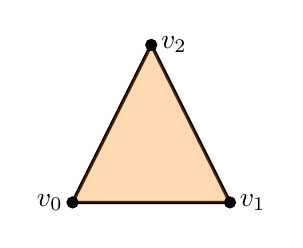
\begin{tikzpicture} %Un 2-simplejo
        \coordinate (A) at (0,0);
        \coordinate (B) at (2,0);
        \coordinate (C) at (1,2);

        \draw[very thick] (A) -- (B) -- (C) -- cycle;
        \fill[color=orange, opacity=0.3] (A) -- (B) -- (C) -- cycle;

        \filldraw (C) circle (2pt) node[anchor=west]{$v_{2}$};
        \filldraw (B) circle (2pt) node[anchor=west]{$v_{1}$};
        \filldraw (A) circle (2pt) node[anchor=east]{$v_{0}$};
    \end{tikzpicture}
\end{center}

\vspace{2mm}
\begin{dfn}
    Un \textbf{complejo simplicial} (geométrico) $K$ es un conjunto de simplejos tales que
    \begin{enumerate}
        \item Si $\sigma\in K$ y $\tau\leq\sigma$ entonces $\tau\in K$.
        \item Si $\sigma,\tau\in K$ entonces $\sigma\cap\tau=\emptyset$ ó $\sigma\cap\tau$ es una
        cara de $\sigma$ y de $\tau$.
    \end{enumerate}
\end{dfn}
\noindent El \textbf{poliedro} asociado a un complejo simplicial $K$ es 
$\abs{K}:=\bigcup_{\sigma\in K}\sigma$. Un espacio topológico $X$ se llama un poliedro si existe
un complejo simplicial $K$ y un homeomorfismo $f:\abs{K}\to X$. Al par $(K,f)$ se le llama una 
\textbf{triangulación} de $X$. Denotamos por $V_{K}$ al conjunto de vértices de los simplices.

\vspace{2mm}
\noindent\textbf{Observación:} Si $X$ es triangulable, entonces es Hausdorff por que $\abs{K}$ 
lo es.

\begin{center}
    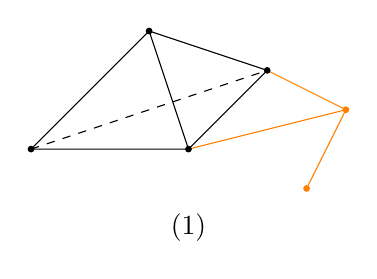
\begin{tikzpicture} %Ejemplo de complejo simplicial
        \coordinate (A) at (0,0);
        \coordinate (B) at (2,0);
        \coordinate (C) at (3,1);
        \coordinate (D) at (1.5,1.5);
        \coordinate (E) at (4,0.5);
        \coordinate (F) at (3.5,-0.5);

        \draw (A) -- (B) -- (D) -- cycle;
        \draw (D) -- (C) -- (B);
        \draw[dashed] (A) -- (C);
        \draw[color=orange] (B) -- (E) -- (C);
        \draw[color=orange] (E) -- (F);

        \filldraw (A) circle (1pt);
        \filldraw (B) circle (1pt);
        \filldraw (C) circle (1pt);
        \filldraw (D) circle (1pt);
        \filldraw[color=orange] (E) circle (1pt);
        \filldraw[color=orange] (F) circle (1pt);

        \node at (2,-1) {(1)};
    \end{tikzpicture}
    %
    \hspace{2cm}
    %
    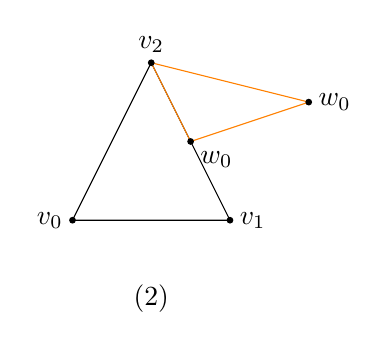
\begin{tikzpicture} %Ejemplo de un no complejo simplicial
        \coordinate (A) at (0,0);
        \coordinate (B) at (2,0);
        \coordinate (C) at (1,2);
        \coordinate (D) at (1.5,1);
        \coordinate (E) at (3,1.5);

        \draw (A) -- (B) -- (C) -- cycle;
        \draw[color=orange] (C) -- (D) -- (E) -- cycle;

        \filldraw (A) circle (1pt) node[anchor=east]{$v_{0}$};
        \filldraw (B) circle (1pt) node[anchor=west]{$v_{1}$};
        \filldraw (C) circle (1pt) node[anchor=south]{$v_{2}$};
        \filldraw (D) circle (1pt) node[anchor=north west]{$w_{0}$};
        \filldraw (E) circle (1pt) node[anchor=west]{$w_{0}$};

        \node at (1,-1) {(2)};
    \end{tikzpicture}
\end{center}
\noindent La figura $(1)$ corresponde a un complejo simplicial, mientras que la figura $(2)$ no
es un complejo simplicial ya que los simplices que la componen no se pegan bien.

\vspace{2mm}
\noindent\textbf{Ejemplo:} Consideremos el complejo simplicial $K$ formado por los simplices 
$\sigma=\gen{\pm e_{1},\pm e_{2}, \pm e_{3}}$ y sus respectivas caras. Consideremos 
$f:\abs{K}\to\s^{2}$ por $f(x):=x/\abs{x}$, entonces $(K,f)$ es una triangulación de la 
$2-$esfera.

\begin{center}
    \begin{tikzpicture}[scale=0.9] %Representación del complejo simplicial
        \coordinate (O) at (0,0);
        \coordinate (A) at (-0.5,-1);
        \coordinate (B) at (1,0);
        \coordinate (C) at (0,1);

        \draw (O) -- ($1.5*(A)$);
        \draw (O) -- ($1.5*(B)$);
        \draw (O) -- ($1.5*(C)$);

        \draw[dashed] (O) -- ($-1.5*(A)$);
        \draw[dashed] (O) -- ($-1.5*(B)$);
        \draw[dashed] (O) -- ($-1.5*(C)$);

        \draw[orange] (A) -- (B) -- (C) -- cycle;
        \draw[orange] (A) -- (B) -- ($-1*(C)$) -- cycle;
        \draw[orange] (A) -- ($-1*(B)$) -- (C) -- cycle;
        \draw[orange] ($-1*(A)$) -- (B) -- (C) -- cycle;

        \draw[orange, dashed] ($-1*(B)$) -- ($-1*(C)$);
        \draw[orange, dashed] ($-1*(B)$) -- ($-1*(A)$);
        \draw[orange, dashed] ($-1*(A)$) -- ($-1*(C)$);

        \filldraw (A) circle (1pt) node[anchor=north west]{$e_{1}$};
        \filldraw (B) circle (1pt) node[anchor=north west]{$e_{2}$};
        \filldraw (C) circle (1pt) node[anchor=south west]{$e_{3}$};
    \end{tikzpicture}
\end{center}

\vspace{2mm}
\begin{dfn}
    Sean $K$ y $L$ complejos simpliciales. Un \textbf{mapeo simplicial} de $K$ a $L$ es una 
    función $f:V_{K}\to V_{L}$ tal que si $\sigma=\gen{v_{\alpha_{0}},\cdots,v_{\alpha_{n}}}$ es
    un simplejo en $K$ entonces
    \begin{equation*}
        \{f(v_{\alpha_{0}}),\cdots,f(v_{\alpha_{n}})\}
    \end{equation*}
    genera un simplice en $L$, al cual llamamos $f(\sigma)$. Notación $f:K\to L$.
\end{dfn}

\vspace{2mm}
\noindent\textbf{Ejemplo:} Sea $\triangle^{n}=\gen{e_{1},\cdots,e_{n+1}}\subseteq\R^{n+1}
\subseteq\R^{\infty}$. Entonces las funciones $f:\triangle^{1}\to\triangle^{2}$ y 
$g:\triangle^{2}\to\triangle^{1}$ dadas por $f(e_{i})=e_{i}$ y $g(e_{1})=g(e_{3})=e_{1}$, 
$g(e_{2})=e_{2}$ son mapeos simpliciales.

\vspace{2mm}
\begin{lema}
    Sea $f:K\to L$ un mapeo simplicial. Entonces induce una función continua 
    $\abs{f}:\abs{K}\to\abs{L}$.
\end{lema}
\begin{proof}
    Sea $\sigma\in K$, digamos que $\sigma=\gen{v_{\alpha_{0}},\cdots,v_{\alpha_{n}}}$ y Definimos
    \begin{align*}
        f_{\sigma}:\sigma &\to \abs{L} \\
        \sum_{i=0}^{k}t_{i}v_{i} &\to \sum_{i=0}^{k}t_{i}f(v_{i})
    \end{align*}
    que es continua por que es lineal en los $t_{i}$. Se observa que si $\tau\leq\sigma$ entonces
    $f_{\tau}=f_{\sigma}\big|_{\tau}$. Ahora tomamos $\sigma$ y $\sigma'$, entonces
    \begin{equation*}
        f_{\sigma}\big|_{\sigma\cap\sigma'}=f_{\sigma\cap\sigma'}
        =f_{\sigma'}\big|_{\sigma\cap\sigma'}
    \end{equation*}
    entonces $\abs{f}:=\bigcup_{\sigma\in K}f_{\sigma}$ es una función continua de $\abs{K}$ en 
    $\abs{L}$.
\end{proof}
\noindent Sea $g:L\to J$ un mapeo simplicial, entonces $g\circ f$ es mapeo simplicial, ya que $f$
mapea vértices de un simplice a vértices de un simplice y del mismo modo lo hace $g$, además se 
tiene lo siguiente
\begin{equation*}
    \abs{g\circ f}(x)=\abs{g\circ f}\left(\sum t_{i}v_{\alpha_{i}}\right)
    =\sum t_{i}(g\circ f)(v_{\alpha_{i}})=\sum t_{i}g(f(v_{\alpha_{i}}))=(\abs{g}\circ\abs{f})(x)
\end{equation*}
es decir, $\abs{g\circ f}=\abs{g}\circ\abs{f}$. Un mapeo simplicial puede ser definido también 
como una función continua $f:\abs{K}\to\abs{L}$ que manda vértices en vértices y es lineal en sus 
caras.

\vspace{2mm}
\noindent Daremos un par de definiciones útiles para mas adelante, que están relacionadas con la 
noción de aproximar una función continua por un mapeo simplicial.

\vspace{2mm}
\begin{dfn}
    Sea $x\in\abs{K}$. El \textbf{portador} de $x$ es el simplejo de $K$ mas pequeño (en términos
    de inclusión) que contiene a $x$. Se denota por $carr(x)$.
\end{dfn}
\noindent\textbf{Ejemplo:} Veamos el siguiente complejo
\begin{center}
    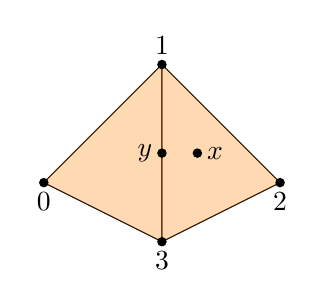
\begin{tikzpicture}[scale=1.5] %Ejemplo concreto del portador
        \coordinate (O) at (0,0);
        \coordinate (A) at (1,0.5);
        \coordinate (B) at (-1,0.5);
        \coordinate (C) at (0,1.5);

        \draw (O) -- (A) -- (C) -- cycle;
        \draw (O) -- (B) -- (C) -- cycle;

        \fill[color=orange, opacity=0.3] (O) -- (A) -- (C) -- cycle;
        \fill[color=orange, opacity=0.3] (O) -- (B) -- (C) -- cycle;

        \filldraw (B) circle (1pt) node[anchor=north]{$0$};
        \filldraw (A) circle (1pt) node[anchor=north]{$2$};
        \filldraw (O) circle (1pt) node[anchor=north]{$3$};
        \filldraw (C) circle (1pt) node[anchor=south]{$1$};

        \filldraw (0,0.75) circle (1pt) node[anchor=east]{$y$};
        \filldraw (0.3,0.75) circle (1pt) node[anchor=west]{$x$};
    \end{tikzpicture}
\end{center}
Entonces $carr(y)=\gen{1,3}$, $carr(x)=\gen{1,2,3}$ y $carr(4)=\gen{4}$.

\vspace{2mm}
\noindent\textbf{Observación:} Notemos que $y\in carr(x)$ si y solo si $carr(y)\subseteq carr(x)$.
Sea $\sigma\in K$, entonces $\sigma=carr(x)$ si y solo si $x\in int(\sigma)$, esto es una 
caracterización útil del portador.

\vspace{2mm}
\noindent En efecto, si $\sigma=carr(x)$, supongamos, por contradicción, que $x\in\partial\sigma$,
entonces $x\in\tau<\sigma$, como $K$ es complejo, $\tau\in K$. Por otro lado, si 
$x\in int(\sigma)$, sea $\tau\in K$ tal que $x\in\tau$, luego $\tau\cap\sigma$ es una cara de 
$\sigma$, pero $x\in\tau\cap\sigma$ lo que implica que $\sigma=\tau\cap\sigma\subseteq\tau$, es
decir, $\sigma=carr(x)$.

\vspace{2mm}
\begin{prop}
    Sea $g:K\to L$ un mapeo simplicial, entonces $g(carr(x))=carr(g(x))$.
\end{prop}
\begin{proof}
    Por la observación anterior, basta probar que $g(x)\in int(g(carr(x)))$, sean $v_{i}\in V_{K}$
    tales que $\gen{v_{1},\cdots,v_{n}}=carr(x)$, luego
    \begin{equation*}
        x=\sum_{i=1}^{n}t_{i}v_{i}\htext{donde}t_{i}>0\text{ para todo }i\text{, entonces}
        \hspace{4mm}g(x)=\sum_{i=0}^{n}t_{i}g(v_{i})\in g(carr(x))
    \end{equation*}
    como $t_{i}>0$ vemos que $g(x)\in int(g(carr(x)))$.
\end{proof}

\begin{dfn}
    Sea $f:\abs{K}\to\abs{L}$ una función continua. Una \textbf{aproximación simplicial} a $f$ es 
    un mapeo simplicial $g:K\to L$ tal que
    \begin{equation*}
        g(x)\in carr(f(x))\text{ para todo }x\in\abs{K}
    \end{equation*}
\end{dfn}
\noindent\textbf{Ejemplo:} Se definen los siguientes complejos simpliciales,
\begin{center}
    \begin{tikzpicture} %Complejo simplicial K%
        \coordinate (A) at (1,0);
        \coordinate (B) at ({sqrt(2)/2},{sqrt(2)/2});
        \coordinate (C) at (0,1);
        \coordinate (D) at (-{sqrt(2)/2},{sqrt(2)/2});
        \coordinate (E) at (-1,0);
        \coordinate (F) at (-{sqrt(2)/2},-{sqrt(2)/2});
        \coordinate (G) at (0,-1);
        \coordinate (H) at ({sqrt(2)/2},-{sqrt(2)/2});

        \draw (A) -- (B) -- (C) -- (D) -- (E) -- (F) -- (G) -- (H) -- cycle;

        \filldraw (A) circle (1pt) node[anchor=west]{$v_{0}$};
        \filldraw (B) circle (1pt) node[anchor=south west]{$v_{1}$};
        \filldraw (C) circle (1pt) node[anchor=south]{$v_{2}$};
        \filldraw (D) circle (1pt) node[anchor=south east]{$v_{3}$};
        \filldraw (E) circle (1pt) node[anchor=east]{$v_{4}$};
        \filldraw (F) circle (1pt) node[anchor=north east]{$v_{5}$};
        \filldraw (G) circle (1pt) node[anchor=north]{$v_{6}$};
        \filldraw (H) circle (1pt) node[anchor=north west]{$v_{7}$};

        \filldraw ($(O)-(2,1)$) node{K};
    \end{tikzpicture}
    %
    \hspace{2cm}
    %
    \begin{tikzpicture} %Complejo simplicial L
        \coordinate (A) at (1,0);
        \coordinate (B) at (0,1);
        \coordinate (C) at (-1,0);
        \coordinate (D) at (0,-1);

        \draw (A) -- (B) -- (C) -- (D) -- cycle;

        \filldraw (A) circle (1pt) node[anchor=west]{$w_{0}$};
        \filldraw (B) circle (1pt) node[anchor=south]{$w_{1}$};
        \filldraw (C) circle (1pt) node[anchor=east]{$w_{2}$};
        \filldraw (D) circle (1pt) node[anchor=north]{$w_{3}$};

        \filldraw ($(O)-(2,1)$) node{L};
    \end{tikzpicture}
\end{center}
El poliedro asociado a cada complejo es $\s^{1}$, consideramos la función continua $f(z)=z^{2}$,
una aproximación simplicial es $g(v_{i})=g(v_{i+4})=w_{i}$ para $0\leq i\leq3$.

\vspace{2mm}
\begin{dfn}
    Sea $K$ un complejo simplicial. La \textbf{primera subdivisión baricéntrica $K'$ de $K$} es el 
    complejo simplicial $K'$ cuyos
    \begin{itemize}
        \item Vértices son los baricentros $\hat{\sigma}$ de los simpleces $\sigma$ de $K$.
        \item Un $n-$simplice de $K'$ es 
        $\gen{\hat{\sigma_{0}},\hat{\sigma_{1}},\cdots,\hat{\sigma_{n}}}$ si 
        $\sigma_{0}<\sigma_{1}<\cdots<\sigma_{n}$ (Son caras propias).
    \end{itemize}
    Una $r-$ésima división baricéntrica se define recursivamente $K^{(r)}:=(K^{(r-1)})'$.
    Recordemos que si $\sigma=\gen{v_{0},\cdots,v_{n}}$ entonces 
    $\hat{\sigma}=\frac{1}{n+1}\sum v_{i}$.
\end{dfn}

\vspace{2mm}
\begin{prop}
    Sea $K$ un complejo simplicial entonces $\abs{K'}=\abs{K}$.
\end{prop}

\vspace{2mm}
\noindent\textbf{Ejemplo:} Algunos ejemplos de división baricéntrica de dos simplices.
\begin{center}
    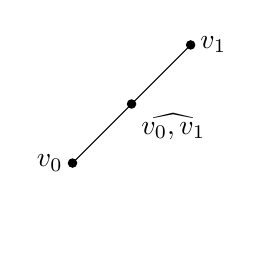
\begin{tikzpicture}[scale=1.5] %División de un 1-simplice
        \coordinate (A) at (0,0);
        \coordinate (B) at (1,1);
        \coordinate (C) at (0.5,0.5);

        \draw (A) -- (B);

        \filldraw (A) circle (1pt) node[anchor=east]{$v_{0}$};
        \filldraw (B) circle (1pt) node[anchor=west]{$v_{1}$};
        \filldraw (C) circle (1pt) node[anchor=north west]{$\widehat{\gen{v_{0},v_{1}}}$};

        \filldraw (0,-0.5) node[]{};
    \end{tikzpicture}
    %
    \hspace{2cm}
    %
    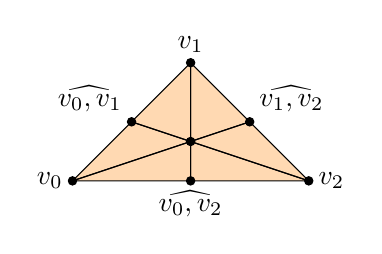
\begin{tikzpicture}[scale=1.5] %División de un 2-simplice
        \coordinate (A) at (-1,0);
        \coordinate (B) at (1,0);
        \coordinate (C) at (0,1);

        \coordinate (D) at (0,0);
        \coordinate (E) at (0.5,0.5);
        \coordinate (F) at (-0.5,0.5);

        \coordinate (G) at (0,{1/3});

        \fill[color=orange, opacity=0.3] (A) -- (B) -- (C) -- cycle;
        
        \draw (A) -- (D) -- (G) -- cycle;
        \draw (A) -- (F) -- (G) -- cycle;

        \draw (B) -- (D) -- (G) -- cycle;
        \draw (B) -- (E) -- (G) -- cycle;

        \draw (C) -- (E) -- (G) -- cycle;
        \draw (C) -- (F) -- (G) -- cycle;

        \filldraw (A) circle (1pt) node[anchor=east]{$v_{0}$};
        \filldraw (B) circle (1pt) node[anchor=west]{$v_{2}$};
        \filldraw (C) circle (1pt) node[anchor=south]{$v_{1}$};

        \filldraw (D) circle (1pt) node[anchor=north]{$\widehat{\gen{v_{0},v_{2}}}$};
        \filldraw (E) circle (1pt) node[anchor=south west]{$\widehat{\gen{v_{1},v_{2}}}$};
        \filldraw (F) circle (1pt) node[anchor=south east]{$\widehat{\gen{v_{0},v_{1}}}$};
        \filldraw (G) circle (1pt);
    \end{tikzpicture}
\end{center}
donde el punto central del segundo ejemplo es $\widehat{\gen{v_{0},v_{1},v_{2}}}$.

\newpage
\subsection{Homología Simplicial}
\noindent Dado $K$ un complejo simplicial finito, esto es, que tiene un número finito de vértices. 
Elegimos un orden total en el conjunto de vértices, digamos $v_{0}<v_{1}<\cdots<v_{n}$.

\vspace{2mm}
\begin{dfn}
    (\textbf{Complejo de cadenas simplicial}) Consideremos los grupos abelianos
    \begin{equation*}
        C_{n}(K):=\left\{\sum n_{\sigma}\sigma:\sigma=\gen{v_{\alpha_{0}},\cdots,v_{\alpha_{n}}}
        \text{ tal que}\hspace{2mm}v_{\alpha_{0}}<\cdots<v_{\alpha_{n}}
        \text{ y}\hspace{2mm}n_{\sigma}\in\Z
        \text{ nulo salvo finitos casos}\right\}
    \end{equation*}
    y los diferenciales $\partial_{n}:C_{n}(K)\to C_{n-1}(K)$ se define en la base por
    \begin{equation*}
        \partial_{n}\gen{v_{\alpha_{0}},\cdots,v_{\alpha_{n}}}
        =\sum_{i=0}^{n}(-1)^{i}\gen{v_{\alpha_{0}},\cdots,\widehat{v_{\alpha_{i}}},
        \cdots,v_{\alpha_{n}}}
    \end{equation*}
    donde $\gen{v_{\alpha_{0}},\cdots,\widehat{v_{\alpha_{i}}},\cdots,v_{\alpha_{n}}}:=
    \gen{v_{\alpha_{0}},\cdots,v_{\alpha_{i-1}},v_{\alpha_{i+1}},\cdots,v_{\alpha_{n}}}$. Se 
    extiende linealmente al resto del grupo.
\end{dfn}

\vspace{2mm}
\begin{teo}
    La tupla $(C_{\sbullet}(K),\partial_{\sbullet})$ es un complejo de cadenas, además, la 
    homología del complejo no depende del orden en el conjunto de vértices.
\end{teo}

\vspace{2mm}
\begin{dfn}
    Sea $K$ un complejo simplicial finito. El \textbf{i-ésimo grupo de homología simplicial} de 
    $K$ es
    \begin{equation*}
        H_{i}(K):=H_{i}(C_{\sbullet}(K))=\frac{\kr{\partial_{i}}}{\im{\partial_{i+1}}}
    \end{equation*}
\end{dfn}

\noindent\textbf{Ejemplos:}
\begin{enumerate}
    \item Sea $K=\{\gen{v_{0},v_{1}},\{v_{0}\},\{v_{1}\}\}$ y consideramos el 
    orden $v_{0}<v_{1}$. El complejo corresponde a un segmento de recta, notemos que 
    $3v_{0}-5v_{1}\in C_{0}(K)$, con la identificación $v_{0}=(1,0)$ y $v_{1}=(0,1)$ vemos que 
    $C_{0}(K)\cong\Z\oplus\Z$, esta identificación no es canónica, es decir, depende de la base 
    que escojamos y sus imagenes correspondientes.

    \vspace{2mm}
    \noindent Por otro lado, $C_{1}(K)\cong\Z$ con la identificación $\gen{v_{0},v_{1}}=1$. 
    Adicionalmente, se tiene que $C_{i}(K)=0$ para $i>1$. Luego,

    \vspace{2mm}
    \centerline{
        \xymatrix{
            0 \ar[r] & C_{1}(K) \ar[r]^{\partial_{1}} & C_{0}(K) \ar[r]^-{0} & 0
        }
    }
    \vspace{2mm}
    \noindent donde $\partial_{1}\gen{v_{0},v_{1}}=v_{1}-v_{2}\in C_{0}(K)$. Con las 
    identificaciones que hicimos resulta que $\partial_{1}(1)=(-1,1)$. De este modo queda la 
    cadena

    \vspace{2mm}
    \centerline{
        \xymatrix{
            0 \ar[r] & \Z \ar[r]^-{\partial_{1}} & \Z\oplus\Z \ar[r]^-{0} & 0
        }
    }
    \vspace{2mm}
    \noindent Así $H_{0}(K)\cong\Z$, $H_{1}(K)=0$, $H_{i}(K)=0$ para $i>0$.

    \item Sean $v_{0},v_{1},v_{2}$ puntos no colineales. Consideramos $\sigma=\gen
    {v_{0},v_{1},v_{2}}$ y $K:=\{\tau\leq\sigma\}$ definimos el orden $v_{0}<v_{1}<v_{2}$. Notemos
    que
    \begin{align*}
        C_{0}(K) &= \Z\{v_{0},v_{1},v_{2}\} \\
        C_{1}(K) &= \Z\{\gen{v_{0},v_{1}},\gen{v_{1},v_{2}},\gen{v_{0},v_{2}}\} \\
        C_{2}(K) &= \Z\{\gen{v_{0},v_{1},v_{2}}\}
    \end{align*}
    Entonces $\partial_{0}=0$,
    \begin{equation*}
        \partial_{1}=\begin{cases}
            \partial\gen{v_{0},v_{1}}=v_{1}-v_{0} \\
            \partial\gen{v_{1},v_{2}}=v_{2}-v_{1} \\
            \partial\gen{v_{0},v_{3}}=v_{3}-v_{0}
        \end{cases}\hhtext{y}
        \partial_{2}\gen{v_{0},v_{1},v_{2}}=\gen{v_{1},v_{2}}-\gen{v_{0},v_{2}}+\gen{v_{0},v_{1}}
    \end{equation*}
    Realizando las identificaciones $v_{i}=e_{i+1}$ para $i=0,1,2$, $\gen{v_{0},v_{1},v_{2}}=1$,
    $\gen{v_{0},v_{1}}=e_{1},\gen{v_{1},v_{2}}=e_{2}$ y $\gen{v_{0},v_{2}}=e_{3}$ resulta que
    $C_{0}(K)\cong\Z^{3},C_{1}(K)\cong\Z^{3}$ y $C_{2}(K)\cong\Z$. Tenemos
    
    \vspace{2mm}
    \centerline{
        \xymatrix{
            \cdots \ar[r] & 0 \ar[r] & C_{2}(K) \ar[r]^{\partial_{2}} & C_{1}(K) 
            \ar[r]^{\partial_{1}} & C_{0}(K) \ar[r] & 0
        }
    }
    \vspace{2mm}
    donde
    \begin{equation*}
        \partial_{2}=\begin{pmatrix}
            1 \\ 1 \\ -1
        \end{pmatrix}
        \hhtext{y}
        \partial_{1}=\begin{pmatrix}
            -1 & 0 & -1 \\ 1 & -1 & 0 \\ 0 & 1 & 1
        \end{pmatrix}
    \end{equation*}

    Claramente $H_{i}(K)=0$ para $i>2$. Además, $\kr{\partial_{2}}$, entonces $H_{2}(K)=0$. 
    Notemos que $\im{\partial_{2}}\cong\Z$ y $\kr{\partial_{1}}\cong\Z$, luego $H_{1}(K)=0$. Por
    otro lado, $\im{\partial_{1}}\cong\Z^{2}$. Por ende $H_{0}(K)\cong\Z$.
\end{enumerate}

\vspace{2mm}
\noindent\textbf{Comentario:} Se invita a calcular la homología de un $n-$simplejo. Hasta ahora 
hemos definido todo respecto a $\Z$, pero se puede definir homología simplicial de manera análoga 
para cualquier anillo $R$.

\vspace{2mm}
\begin{lema}
    Sea $f:K\to L$ un mapeo simplicial, definimos los morfismos
    \begin{align*}
        f_{n}:C_{n}(K) &\to C_{n}(L) \\
        \gen{v_{\alpha_{0}},\cdots,v_{\alpha_{n}}} &\to \begin{cases}
            sign(\varphi)\gen{f(v_{\varphi(\alpha_{0})}),\cdots,f(v_{\varphi(\alpha_{n})})} 
            &\quad\text{ si son distintos} \\
            0 &\quad\text{ si no lo son}
        \end{cases}
    \end{align*}
    donde $\varphi$ es un permutación tal que $\varphi(\alpha_{0})<\cdots<\varphi(\alpha_{n})$. 
    Entonces, la colección, es un mapeo de cadena.
\end{lema}

\noindent Por lo tanto, $f$ induce un morfismo entre los grupos de homología de los complejos
simpliciales

\vspace{2mm}
\noindent\textbf{Ejemplo:} Definimos los siguientes complejos simpliciales
\begin{center}
    \begin{tikzpicture} %Complejo simplicial K%
        \coordinate (O) at (0,0);
        \filldraw[color=black, fill=white, thick] (O) circle (1);
        
        \coordinate (A) at (1,0);
        \coordinate (B) at ({sqrt(2)/2},{sqrt(2)/2});
        \coordinate (C) at (0,1);
        \coordinate (D) at (-{sqrt(2)/2},{sqrt(2)/2});
        \coordinate (E) at (-1,0);
        \coordinate (F) at (-{sqrt(2)/2},-{sqrt(2)/2});
        \coordinate (G) at (0,-1);
        \coordinate (H) at ({sqrt(2)/2},-{sqrt(2)/2});

        \draw (A) -- (B) -- (C) -- (D) -- (E) -- (F) -- (G) -- (H) -- cycle;

        \filldraw (A) circle (1pt) node[anchor=west]{$v_{0}$};
        \filldraw (B) circle (1pt) node[anchor=south west]{$v_{1}$};
        \filldraw (C) circle (1pt) node[anchor=south]{$v_{2}$};
        \filldraw (D) circle (1pt) node[anchor=south east]{$v_{3}$};
        \filldraw (E) circle (1pt) node[anchor=east]{$v_{4}$};
        \filldraw (F) circle (1pt) node[anchor=north east]{$v_{5}$};
        \filldraw (G) circle (1pt) node[anchor=north]{$v_{6}$};
        \filldraw (H) circle (1pt) node[anchor=north west]{$v_{7}$};

        \filldraw ($(O)-(2,1)$) node{K};
    \end{tikzpicture}
    %
    \hspace{2cm}
    %
    \begin{tikzpicture} %Complejo simplicial L
        \coordinate (O) at (0,0);
        \filldraw[color=black, fill=white, thick] (O) circle (1);

        \coordinate (A) at (1,0);
        \coordinate (B) at (0,1);
        \coordinate (C) at (-1,0);
        \coordinate (D) at (0,-1);

        \draw (A) -- (B) -- (C) -- (D) -- cycle;

        \filldraw (A) circle (1pt) node[anchor=west]{$w_{0}$};
        \filldraw (B) circle (1pt) node[anchor=south]{$w_{1}$};
        \filldraw (C) circle (1pt) node[anchor=east]{$w_{2}$};
        \filldraw (D) circle (1pt) node[anchor=north]{$w_{3}$};

        \filldraw ($(O)-(2,1)$) node{L};
    \end{tikzpicture}
\end{center}
Para cada complejo se da el orden que sigue $v_{0}<v_{1}<\cdots<v_{7}$ y $w_{0}<w_{1}<w_{2}<w_{3}$ 
y definimos $f:K\to L$ por $f(v_{i})=f(v_{i+4})=w_{i}$ para $i=0,1,2,3$. Veamos quien es 
$f_{*}:H_{1}(K)\to H_{1}(L)$. En primer lugar, sabemos que
\begin{equation*}
    H_{1}(K)=ker(C_{1}(K)\to C_{0}(K))=ker\begin{pmatrix}
        -1 & 0 & 0 & -1 \\ 1 & -1 & 0 & 0 \\ 0 & 1 & -1 & 0 \\ 0 & 0 & 1 & 1
    \end{pmatrix}=\gen{\begin{pmatrix}
        1 \\ 1 \\ 1 \\ -1
    \end{pmatrix}}\cong\Z
\end{equation*}
Similarmente $H_{1}(K)\cong\Z$. Entonces
\begin{equation*}
    f_{*}(\gen{v_{0},v_{1}}+\cdots+\gen{v_{6},v_{7}}-\gen{v_{0},v_{7}})
    =2(\gen{w_{0},w_{1}}+\gen{w_{1},w_{2}}+\gen{w_{2},w_{3}}-\gen{w_{0},w_{3}})
\end{equation*}
luego $f_{*}:H_{1}(K)\xrightarrow{\cdot2} H_{1}(L)$. Por otro lado, notemos que 
$H_{0}(K)\cong H_{0}(L)\cong\Z$, ya que todo par de vértices en el complejo esta conectado por una
secuencia de aristas, luego $f_{*}([v_{0}])=[w_{0}]$, entonces 
$f_{*}:H_{0}(K)\xrightarrow{} H_{0}(L)$ es isomorfismo.

\vspace{2mm}
\begin{teo}[Mayer-Vietoris]
    Sea $K$ un complejo simplicial y $M,N$ subcomplejos de $K$ que cubren a $K$, es decir, 
    $M\cup N=K$. Se tienen los mapeos
    
    \centerline{
        \xymatrix{
            M\cap N \ar[d]^-{i_{M}} \ar[r]^-{i_{N}} & N \ar[d]^-{j_{N}} \\
            M \ar[r]^-{j_{M}} & K
        }
    }

    \vspace{2mm}
    Existen morfismos $\delta_{n}:H_{n}(K)\to H_{n-1}(K)$ tales que la secuencia

    \centerline{
        \xymatrixcolsep{3pc}\xymatrix{
            \ar[r]^-{\delta_{n+1}} & H_{n}(M\cap N) \ar[r]^-{i_{M*}\oplus i_{N*}} 
            & H_{n}(M)\oplus H_{n}(N) \ar[r]^-{j_{M*}-j_{N*}} & H_{n}(K) 
            \ar `[dl] `[l] `[llld]_{\delta_{n}} `[d] [dll] \\
            & H_{n-1}(M\cap N) \ar[r]^-{i_{M*}\oplus i_{N*}} 
            & H_{n-1}(M)\oplus H_{n-1}(N) \ar[r]^-{j_{M*}-j_{N*}} & H_{n-1}(K) \ar[r] & \cdots \\
            & \cdots \ar[r] & H_{0}(M)\oplus H_{0}(N) \ar[r]^-{j_{M*}-j_{N*}} 
            & H_{0}(K) \ar[r] & 0
        }
    }
    es exacta.
\end{teo}

\begin{proof}
    Verificaremos que
    
    \centerline{
        \xymatrixcolsep{3pc}\xymatrix{
            0 \ar[r] & C_{n}(M\cap N) \ar[r]^-{i_{M}\oplus i_{N}} 
            & C_{n}(M)\oplus C_{n}(N) \ar[r]^-{j_{M}-j_{N}} & C_{n}(K) \ar[r] & 0
        }
    }

    \vspace{2mm}
    es una secuencia exacta corta de grupos abelianos para todo $n\in\N$. En efecto, como $C_{n}$
    es libremente generado por los $n-$simplices e $i$ es inyectiva, entonces 
    $i_{M*}\oplus i_{N*}$ es inyectiva. Además, $j_{M*}-j_{N*}$ es sobreyectiva por hipotesis y
    es directo que $\im{i_{M*}\oplus i_{N*}}\subseteq\kr{j_{M*}-j_{N*}}$. Resta ver que
    \begin{equation*}
        \kr{j_{M*}-j_{N*}}\subseteq\im{i_{M*}\oplus i_{N*}}
    \end{equation*}
    Sea $(x,y)\in\kr{j_{M*}-j_{N*}}$ entonces $j_{M*}(x)=j_{N*}(y)$, es decir, $x$ e $y$ se 
    escriben como suma de simplices en $N$ y $M$ respectivamente, entonces 
    $(x,y)\in\im{i_{M*}\oplus i_{N*}}$. Así, usando el lema de la serpiente, concluimos.
\end{proof}

\noindent\textbf{Ejemplo:}
Consideremos la siguiente situación
\begin{center}
    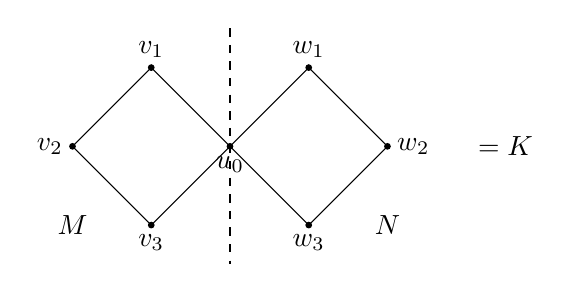
\begin{tikzpicture} %Ejemplo de Mayer Vietoris
        \coordinate (O) at (0,0);
        
        \coordinate (A) at (-1,1);
        \coordinate (B) at (-2,0);
        \coordinate (C) at (-1,-1);

        \coordinate (D) at (1,1);
        \coordinate (E) at (2,0);
        \coordinate (F) at (1,-1);

        \draw (O) -- (A) -- (B) -- (C) -- cycle;
        \draw (O) -- (D) -- (E) -- (F) -- cycle;
        \filldraw (O) circle (1pt) node[anchor=north]{$u_{0}$};
        
        \filldraw (A) circle (1pt) node[anchor=south]{$v_{1}$};
        \filldraw (B) circle (1pt) node[anchor=east]{$v_{2}$};
        \filldraw (C) circle (1pt) node[anchor=north]{$v_{3}$};

        \filldraw (D) circle (1pt) node[anchor=south]{$w_{1}$};
        \filldraw (E) circle (1pt) node[anchor=west]{$w_{2}$};
        \filldraw (F) circle (1pt) node[anchor=north]{$w_{3}$};

        \draw[dashed] (0,1.5) -- (0,-1.5);
        \filldraw (-2,-1) node{$M$};
        \filldraw (2,-1) node{$N$};
        \filldraw (3.5,0) node{$=K$};
    \end{tikzpicture}
\end{center}
Notemos que $H_{1}(M)\cong\Z$ y $H_{1}(N)\cong\Z$, además $M\cap N=\{u_{0}\}$, entonces usando
mayer vietoris nos queda que

\vspace{2mm}
\centerline{
    \xymatrix{
        0 \ar[r] & 0 \ar[r] & \Z\oplus\Z \ar[r] & H_{1}(K) 
        \ar `[dl] `[l] `[llld] `[d] [dll] \\
        & \Z \ar[r]^-{\varphi} & \Z\oplus\Z \ar[r]^{\phi} & H_{0}(K) \ar[r] & 0
    }
}

\vspace{2mm}
\noindent Para $i>2$ notamos que $H_{i}(K)=0$, por otro lado el morfismo $\varphi(1)=(1,1)$ ya que
manda generador en generador, esto por que todo par de puntos en $M$ y $N$ estan relacionados por
un camino de aristas. De este modo,
\begin{equation*}
    H_{0}(K)\cong\frac{\Z\oplus\Z}{\ker{\phi}}=\frac{\Z\oplus\Z}{\im{\varphi}}
    \cong\frac{\Z\oplus\Z}{\Z}\cong\Z
    \hhtext{y}
    H_{1}(K)\cong\Z\oplus\Z
\end{equation*}
donde el último isomorfismo se da por que $\varphi$ es inyectiva, es decir, el morfismo 
$H_{1}(K)\to\Z$ es trivial.

\begin{teo}
    Sea $f:\abs{K}\to\abs{L}$ una función continua. Entonces $f$ induce un homomorfismo
    \begin{equation*}
        f_{*}:H_{*}(K)\to H_{*}(L)
    \end{equation*}
    tal que $(g\circ f)_{*}=g_{*}\circ f_{*}$ e $id_{*}=id_{H_{*}(K)}$, donde 
    $g:\abs{L}\to\abs{M}$ es continua.
\end{teo}

\noindent\textbf{Observación:} Con esto se tendría que $H_{*}(K)$ es invariante topológico. Se
probara en dos pasos. Veremos que toda función $f$ continua se puede ``aproximar'' a una función 
$g$ simplicial, también hay que comprobar que $f_{*}:=g_{*}$ es independiente de la función 
simplicial escogida.

\begin{teo}[Aproximación Simplicial]
    Sean $K,L$ complejos simpliciales finitos y $f:\abs{K}\to\abs{L}$ una función continua. 
    Entonces existe $r\in\N$ y una aproximación simplicial a $f$
    \begin{equation*}
        g:K^{(r)}\to L
    \end{equation*}
\end{teo}

\noindent A partir de esta aproximación simplicial, se cumplen dos propiedades importantes, que 
son
\begin{enumerate}
    \item $f$ es homotópica a $g$. Notemos que $g(x),f(x)\in carr(f(x))$, entonces el segmento 
    entre $g(x)$ y $f(x)$ está en $carr(f(x))$ porque es un conjunto convexo. Definimos
    \begin{align*}
        \abs{K}\times[0,1] &\to \abs{L}\\
        (x,t) &\to tg(x)+(1-t)f(x)
    \end{align*}

    \item Sean $f_{1}:\abs{K}\to\abs{L}$, $f_{2}:\abs{L}\to\abs{M}$ continuas y $g_{1}:K\to L$, 
    $g_{2}:L\to M$ aproximaciones simpliciales de $f_{i}$, entonces $g_{2}\circ g_{1}$ es
    aproximación simplicial de $f_{2}\circ f_{1}$.

    Se tiene que
    \begin{equation*}
        g_{2}g_{1}(x)\in g_{2}(carr(f_{1}(x)))=carr(g_{2}f_{1}(x))\subseteq carr(f_{2}f_{1}(x))
    \end{equation*}
\end{enumerate}

\begin{prop}
    Sea $id:\abs{K'}\to\abs{K}$, la función $a:V_{K'}\to V_{K}$ dada por 
    $a(\hat{\sigma})=v\in V_{\sigma}$ cumple que
    \begin{enumerate}
        \item Define una aproximación simplicial de la identidad.
        \item Toda aproximación simplicial $g:K'\to K$ de la identidad es de esta forma.
    \end{enumerate}
\end{prop}

\begin{proof}
    Veamos que $a$ es un mapeo simplicial. Sea $\sigma
    =\gen{\hat{\sigma_{0}},\cdots,\hat{\sigma_{n}}}\in K'$, entonces 
    $a(\hat{\sigma_{i}})=v_{i}\in V_{\sigma_{i}}$. Sabemos que $\sigma_{i}<\sigma_{i+1}$
    para $0\leq i\leq n-1$, lo que implica que $V_{\sigma_{i}}\subset V_{\sigma_{i+1}}$, en 
    particular, $V=\{v_{0},\cdots,v_{n}\}\subseteq V_{\sigma_{n}}$, luego, $V$ genera una cara de 
    $\sigma_{n}$, es decir, un simplice en $\abs{K}$.

    \vspace{2mm}
    Sea $x\in\abs{K'}$, sean $\hat{\sigma_{i}}\in K'$ tales que 
    $\gen{\hat{\sigma_{1}},\cdots,\hat{\sigma_{n}}}=carr(x)$, luego,
    \begin{equation*}
        x=\sum_{i=1}^{n}t_{i}\hat{\sigma_{i}}\htext{donde}t_{i}>0\text{ para todo }i
    \end{equation*}
    en particular, $t_{n}>0$, como $\hat{\sigma_{n}}=\frac{1}{n+1}\sum v_{i}$ donde 
    $\gen{v_{1},\cdots,v_{n}}=\sigma_{n}$, entonces $x$ se escribe como combinación convexa de los
    $v_{i}$ donde cada poderación es positiva, luego $x\in int(\sigma_{n})$, en otras palabras,
    $carr(id(x))=\sigma_{n}$.

    \vspace{2mm}
    Lo anterior prueba que $a$ es una aproximación de la identidad. Por otro lado, si $g$ es una
    aproximación simplicial de la identidad, entonces
    \begin{equation*}
        g(\hat{\sigma})\in carr(id(\hat{\sigma}))=\sigma
    \end{equation*}
    entonces $g(\hat{\sigma})\in V_{\sigma}$, por que $g$ es mapeo simplicial.
\end{proof}

\vspace{2mm}
\begin{lema}
    Si $f,g:K\to L$ son aproximaciones simpliciales de alguna función continua $\abs{K}\to\abs{L}$
    entonces $g_{*}=f_{*}$.
\end{lema}

\vspace{2mm}
\begin{lema}
    Sea $a:K'\to K$ una aproximación simplicial de $id:\abs{K'}\to\abs{K}$. Entonces 
    $a_{*}:H_{n}(K')\to H_{n}(K)$ es un isomorfismo para todo $n\in\N$.
\end{lema}

\noindent Si iteramos, $a_{r}:K^{(r)}\to K$ entonces $a_{r*}:H_{n}(K^{(r)})\to H_{n}(K)$ es 
isomorfismo para todo $n\in\N$.

\begin{teo}
    Sea $f:\abs{K}\to\abs{L}$ una función continua, entonces el homomorfismo
    \begin{equation*}
        f_{*}:=s\circ a_{r*}^{-1}:H_{n}(K)\to H_{n}(L)
    \end{equation*}
    donde $s$ es aproximación simplicial de $f$. Cumple que
    \begin{enumerate}
        \item No depende de $s$ ni de $r$.
        \item Si $g:\abs{L}\to\abs{M}$ es continua, entonces $(f\circ g)_{*}=f_{*}\circ g_{*}$.
    \end{enumerate}
\end{teo}
\noindent La demostración de $(1)$ es inmediata de los dos lemas previos y $(2)$ es directo de la
segunda propiedad que se tiene del teorema de aproximación simplicial. Con esto, ya podemos 
afirmar que la homología simplicial es un invariante topológico.

\newpage
\subsection{Homología Singular}

\newpage
\subsection{Homología Relativa}

\newpage
\subsection{Resultados de Homología}

\newpage
\section{Cohomología}

\subsection{Complejos de Cocadenas}

\newpage
\subsection{Cohomología Singular y Simplicial}

\newpage
\subsection{Producto Cup}

\newpage
\subsection{Anillo de Cohomología}

\newpage
\subsection{Dualidad de Poincaré y Fórmula de Künneth}

\newpage
\section{Grupo Fundamental}

\subsection{Primer Grupo Fundamental}

%\printbibliography % Quitar el comentado si quiero usar bibliografia

\end{document}